%カタクチ対馬

%タイトル

\chapter*{\ThisFiscalYr(\ThisYrAD)年度カタクチイワシ対馬暖流系群の資源評価}

%基礎情報

\begin{table}[h]

  \begin{tabular}{{rp{14cm}}}

責任担当水研: &西海区水産研究所 (安田十也、林 晃、黒田啓行、髙橋素光)\\

参画機関: & 日本海区水産研究所、青森県産業技術センター水産総合研究所、秋田県水産振興センター、山形県水産試験場、新潟県水産海洋研究所、富山県農林水産総合技術センター水産研究所、石川県水産総合センター、福井県水産試験場、京都府農林水産技術センター海洋センター、兵庫県立農林水産技術総合センター但馬水産技術センター、鳥取県水産試験場、島根県水産技術センター、山口県水産研究センター、福岡県水産海洋技術センター、佐賀県玄海水産振興センター、長崎県総合水産試験場、熊本県水産研究センター、鹿児島県水産技術開発センター

  \end{tabular}

\end{table}

%要約

\begin{center}\Large{{\gt 要   約}}\end{center}

%内容

本系群の資源量について、コホート解析により計算した。資源量は1995年から2000年まで200千トン以上であったが、2001年に130千トンへ減少した。2004年以降資源量は増加し、2007年には247千トンとなったが、それ以降減少傾向を示した。2015年における資源量は132千トンと推定され、前年(120千トン)より増加した。過去の資源量と親魚量から資源水準は低位、過去5年間(2011~2015年)の資源量の推移から動向は横ばいと判断した。再生産関係から、Blimitを2005年水準の親魚量91千トンとした。2015年の親魚量(61千トン)はBlimitを下回っている。5年後に親魚量をBlimitまで回復させるF(Frec5yr)を管理基準値として、2017年ABCを算出した。ただし、本報告でのABCは仔魚(シラス)を含む日本の漁獲に対する値である。

%管理値の表

%水準と動向

%データセットに関する表

%内容

\subsection{まえがき}

\subsection{生態}

\subsubsection{分布・回遊}

«カタクチイワシは、日本海では日本、朝鮮半島、沿海州の沿岸域を中心に分布する(落合・田中 1986)。過去には、日本海の中央部や間宮海峡以南の北西部でも分布が確認されている(ベリャーエフ・シェルシェンコフ 未発表)。東シナ海では、日本、朝鮮半島、中国の沿岸域を中心にして、沖合域にも分布することが報告されている(図1、Iversen et al. 1993、 Ohshimo 1996)。日本漁船の主漁場は日本海西部および九州北~西岸の沿岸域である。
  日本海および東シナ海におけるカタクチイワシの詳細な回遊経路は不明である。卵の出現状況からみて、対馬暖流域の産卵は、主に春から夏にかけて対馬暖流の影響下にある水域で行われ、能登半島以南の水域ではさらに秋季まで継続すると考えられる(内田・道津 1958)。

\subsubsection{年齢・成長}

本系群の成長様式は、発生時期によって異なることが知られている。本報告では、耳石に形成される日周輪の解析結果および体長組成の経月変化から、孵化した個体が半年後には被鱗体長で約9 cmまで成長すると仮定した。体長組成の経月変化から、春季と秋季の発生群について成長様式を求めたところ、次のような結果を得た(図2、大下 2009)。
春季発生群:
	秋季発生群:
ただし、BLtは孵化後tヶ月の被鱗体長(mm)である。
 寿命は3年程度と考えられている。


\subsubsection{成熟・産卵}

カタクチイワシは、厳冬期を除いて周年にわたり産卵することが知られている。若狭湾では体長8.5 cmで産卵することが報告されている(Funamoto et al. 2004)。鳥取県沿岸においては、体長11.9 cm以上であれば、ほとんどが産卵すると報告されている(志村ほか 2008)。これらの結果に従えば、春季発生群は翌年の産卵期にほぼ全て産卵することとなる。そのため、本報告では満1歳から全個体が産卵に参加すると仮定した(図3)。

\subsubsection{被捕食関係}

カタクチイワシは、動物プランクトンのうち主にカイアシ類を餌料とする(Tanaka et al. 2006)。本種は多様な動物種の餌料となっており、仔稚魚期にはマアジ・マサバなどの魚食性魚類や肉食性動物プランクトンに、未成魚・成魚期には魚食性魚類の他に、クジラやイルカなどの海産ほ乳類や海鳥類などにも捕食される。


\subsection{漁業の状況}

\subsubsection{漁業の概要}

本系群は、日本海北区(石川県から新潟県)では主に定置網により漁獲され、日本海西区(福井県から山口県)では主に大中型まき網・中型まき網・定置網などにより漁獲されている。また、東シナ海区(福岡県から鹿児島県)では、主に中型まき網により漁獲される。なお、シラスは主に熊本県や鹿児島県の沿岸域で漁獲されている。


\subsubsection{漁獲量の推移}

本系群の漁獲量は、漁業・養殖業生産統計年報の青森県~鹿児島県の合計値から、東シナ海区に所属する漁船による太平洋海域における漁獲量(漁獲成績報告書による)を差し引いた値とした(表1、図4)。本系群の漁獲量は、1997年を除いて1996年から2000年までは100千トンを超えていたが、その後2004年には61千トンにまで減少した。漁獲量は2005年から2008年にかけて再び増加したが、2009年以降は減少傾向にあり、2015年は61千トンであった。
 海区別では、日本海北区の漁獲量は1995年に9千トンまで増加した後、1996年、2001年、2005年を除いて5千トン前後で変動していたが、2011年から2013年にかけて3千トンを下回った(表1)。2015年の漁獲量は3千トンであった。
日本海西区の漁獲量は、1991年から1998年にかけて70千トンまで増加したが、その後減少し、2001年以降は20千トン前後で推移した。2015年は11千トンと少なかった(表1)。
東シナ海区の漁獲量は、1990年から2000年(65千トン)まで増加傾向にあった。その後は、2009年(26千トン)を除いて、2001から40~70千トンで推移しており、2015年は47千トンであった(表1)。
対馬暖流域の沿岸域における仔魚(シラス)の漁獲量は、1977年以降1987年まで2千トンから6千トンの間で緩やかに増減したが、それ以降10年間ほど6千トン前後の漁獲が維持された(表1)。漁獲量は1999年と2000年には10千トンを超えたが、2002年にかけて急減した。漁獲量はその後、2005年前後に再び10千トン近くまで増加したが、2008年以降から減少傾向を示し、2015年には5千トンとなった。
韓国におけるカタクチイワシ漁獲量は、1995年以降20万トンを超えており、2000年以降は増減を繰り返している(表1;水産統計(韓国海洋水産部)、http://www.fips.go.kr:7001/index.jsp、2016年3月)。2015年における漁獲量は21万トンであった。韓国近海の漁場は韓国南岸および東岸である(韓国国立水産振興院 2000)。中国の漁獲量は、日本・韓国よりも多く、1996年以降50万トン以上で維持されているが、2003年に約111万トンとなって以降、2009年まで減少が続いた(FAO Fishery and Aquaculture Statistics. Global capture production 1950-2014、http://www.fao.org/fishery/statistics/software/fishstatj/en、2016年6月)。中国の漁獲量は2009年以降増加しており(表1)、データが利用可能な直近年である2014年における値は93万トンであった。


\subsection{資源の状態}

\subsubsection{資源評価の方法}

シラスを含めた年別年齢別漁獲尾数に基づくコホート解析により資源量を推定した(補足資料2)。産卵量調査、計量魚探調査および新規加入量調査(ニューストンネット)などの結果は、資源量を反映しているかの検討が不十分なため、コホート解析における資源量指標値としては用いず、資源動向などを判断するための参考値に留めた。

\subsubsection{資源量指標値の推移}

日本海と東シナ海における産卵量の推移を図5に示す。産卵量は1998~2000年に多く、2001年には少なかったものの、2004年には合計10,084兆粒と1979年以降における最大値を示した。その後、産卵量は増減を繰り返している。2015年における産卵量の水準は日本海および東シナ海ともに中程度で、合計値は2,471兆粒であった。
夏季(8・9月)に九州北西岸で行われている、音響調査による現存量指標値(Ohshimo 2004)および中層トロール調査のCPUE(漁獲尾数÷有効網数)を図6に示す。現存量指標値は増減を繰り返しながら推移しており、近年では2007年の134.0(相対値)が最も高かった。現存量指標値はその後、急減し、2010~2012年は2.5~17.9と低水準で推移した。2013年の現存量指標値は2007年の値の半分を超える程度まで回復し、2015年は108.8となった。また、中層トロール調査のCPUEは、1990年代後半に比べると、2002年以降は低水準で変動している。2015年のCPUEは67.4(kg/網)で、前年の値(12.3 kg/網)を大きく上回った。
九州北西岸で実施した調査において、ニューストンネットに入網したシラスのCPUEの推移を図7に示した。6月に実施した調査におけるCPUEは、2003年(598尾/網)、2005年(815尾/網)、2009~2011年(475~928尾/網)に高い値を示したが、2012年以降には299尾/網以下と低い水準にある。8・9月の調査では、CPUEは2010年から2013年にかけて4~25尾/網と低い水準にあったが、2014年は214尾/網と大きく増加した。しかし、2015年には67尾/網となり、前年を下回った。その他主要魚種の採集個体数と、それに対応する有効曳網数は補足資料5に示した。
4月に東シナ海で実施した調査において、ニューストンネットに入網したシラスのCPUEの推移を図8に示した。2003~2007年における値(385~765尾/網)に比べると、2008年~2010年は28~93尾/網と低い水準にあったが、2011年以降増加傾向を示し、2015年には大幅に増加して1622尾/網となった。2015年は前年を下回り955尾/網であった。

\subsubsection{漁獲物の年齢組成}

本系群の年齢別漁獲尾数の推移を図9と表2に示した。漁獲物のほとんどは0歳魚で、0歳魚の漁獲尾数には1977年以降、緩やかな増減が見られる。0歳魚の漁獲尾数は、近年では1990年代後半と2000年代半ばに多かった。


\subsubsection{資源量と漁獲割合の推移}

コホート解析(補足資料2)を用いて、本系群の資源尾数・漁獲係数(表3)及び資源量・親魚量・再生産成功率RPS(加入尾数÷親魚量)・漁獲割合(漁獲量÷資源量)(表4、図10)を推定した。1977年以降における資源量の最低値は1979年における74千トンであり、資源量はその後、増減を繰り返しながらも徐々に増加した。資源量は1998年に306千トンの最大値を記録したが、2001年には130千トンにまで減少した。資源量はその後、2007年まで再び増加傾向を示したが、2008年以降には減少傾向にある。2015年の資源量は132千トンで、前年(120千トン)より増加したものの1987年以来の低水準であった。漁獲割合は、1977年以降50%前後で推移し、2015年の値は50%だった。
 自然死亡係数(M)を0.5、1.0(規定値)、1.5とした場合の資源量・親魚量・加入尾数の推定値を図11に示した。資源量は、Mを0.5に仮定した場合には規定値の72%となり、Mを1.5に仮定した場合には144%となった。


\subsubsection{Blimitの設定}

親魚量と加入尾数との関係を図12に示した。親魚量と加入尾数は正の相関を示した。RPSの上位10%と加入尾数の上位10%にそれぞれ相当する2直線の交点から、資源回復の閾値となるBlimitを親魚量91千トン(2005年水準)とした。2015年の親魚量は61千トンであり、Blimitを下回っている。親魚量と加入量の経年変化を図13に、RPSの経年変化を図14に示した。RPSは増減を繰り返しながらも周期的な変化がみられる。
 F(各年齢のFの平均値)とYPRおよび%SPRの関係を図15に示した。2015年のF(2.48)はFmed(2.12)やF30%SPR(1.29)、Fmax(0.91)、F0.1(0.60)よりも高い。


\subsubsection{資源の水準・動向}

Blimitである親魚量(91千トン)を資源水準の「低位」と「中位」の境界とした。また親魚量の最小値を基準とした場合に、親魚量の最大値までの増分の上位1/3と2/3の境界(155千トン)を「高位」と「中位」の境界とした。なお、同様の方法において下位1/3にあたる親魚量は100千トンで、これはBlimitに比較的近似している。2015年の親魚量(61千トン)がBlimitを下回っていることから、資源の水準を低位と判断した。動向は、過去5年(2011年~2015年)の資源量と親魚量の推移から横ばいと判断した。


\subsubsection{資源と漁獲の関係}

資源量と漁獲係数(F)との間に明瞭な関係は見られなかった(図16)。

\subsection{\ThisYrAD 年ABCの算定}

\subsubsection{資源評価のまとめ}

コホート解析によると2015年の親魚量は61千トンであり、これは再生産関係(図12)から求められるBlimit(親魚量91千トン)を下回っている。資源量と親魚量はともに2011年以降、横ばい傾向にある。以上を根拠に、資源水準を低位、動向を横ばいと判断した。

\subsubsection{ABCの算定}

ABCの表

\subsubsection{ABCの評価}

Fcurrentを変化させた表

\subsubsection{ABCの再評価}

データ追加や修正に関する表

再評価の表

\subsection{ABC以外の管理方策の提言}

\subsection{引用文献}

%図

分布・回遊

\begin{figure}[H]

Subtopic 1

\begin{center}

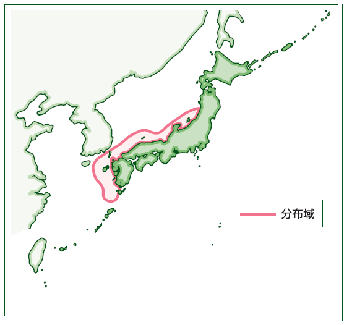
\includegraphics{bunpu.pdf}

\caption{カタクチイワシ対馬暖流系群の分布域    
}

\label{bunpu}

\end{center}

\end{figure}

年齢・成長と年齢別成熟割合

農林大海区と調査点

産卵状況

海区別漁獲量

努力量あたり漁獲量

年間産卵量

%表
